\section{Introduction}\label{sec:intro}

{\em ``Over and above the actual world there are an indefinite multiplicity
of merely possible worlds... The actual world is a possible world. The other
possible worlds, the merely possible worlds, are ways that the actual world
might have been.''} \cite{Armstrong89:worlds} -- D.M. Armstrong

\vspace*{3mm}
% Motivation.
% At a high level, what is the problem area you are working in?
% Why is it important?
% Why is the problem of interest and importance to the larger community?
Traditional concurrent programs are typically subjected to blocking and race
conditions. The exact runtime behavior is often {\em nondeterministic}
because the actual mechanism of the (operating system) scheduler is
{\em unknown} or too complex to the programmer {\em a priori}.
%But in reality, for a given scheduler, a particular runtime environment
%and a given concurrent program, the serial schedule or the interleaving
%is deterministic.
It is easy to write a concurrent
program that leads to deadlock or starvation --  not
achieving termination and desired goals.

\begin{figure}[bh]
\centering
%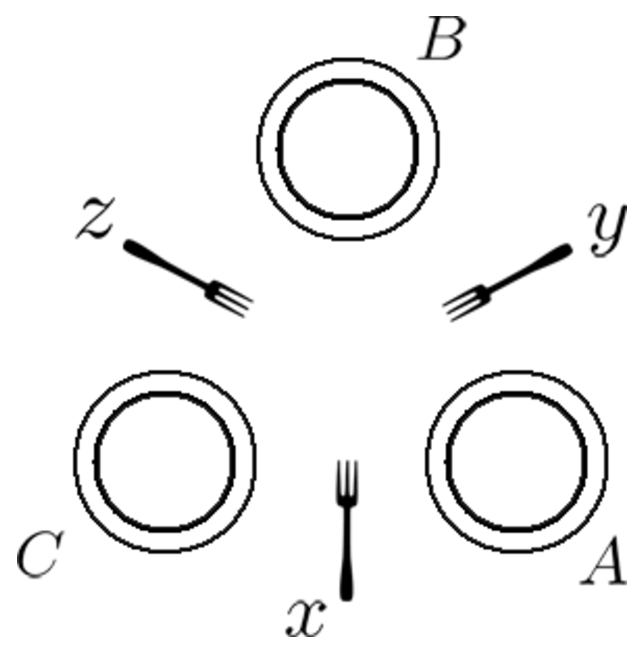
\includegraphics[width=0.2\textwidth]{dining.eps}
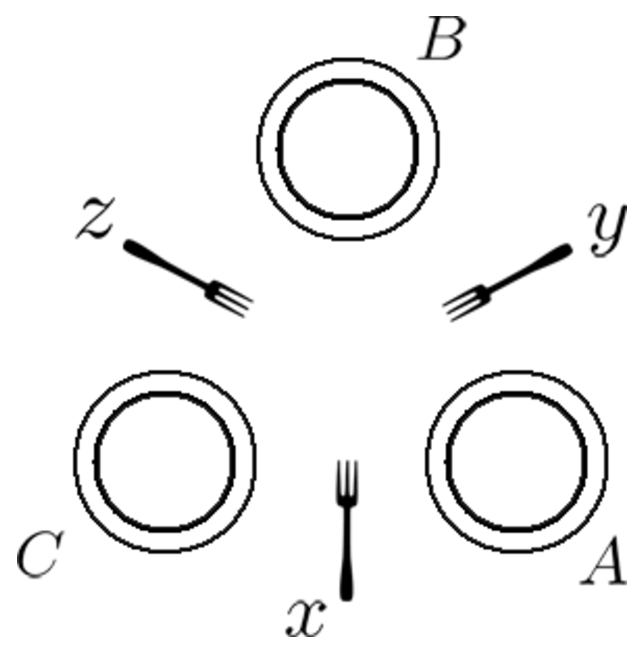
\epsfig{file=dining.eps,width=0.3\columnwidth}
\caption{Three Dining Philosophers Problem}
\label{fig:dining}
\end{figure}

Consider the well-known ``Dining Philosophers Problem''
\cite{Dijkstra2002:Hierarchical} 
- there are three
philosophers $A$, $B$ and $C$, sitting around a dining table,
with three forks $x$, $y$ and $z$ between them,
as shown in \figref{fig:dining}. This classic concurrency problem
shows that deadlock happens with certain sequences of acquiring the forks,
e.g., $A$ acquires $x$, $B$ acquires $y$ and then
$C$ acquires $z$. 
% Consequently, all three philosophers are blocked.
The classic solution to this problem is using a synchronization mechanism 
such as a counting semaphore, imposing a partial order on acquiring the forks, 
or requiring one philosopher to be asymmetric.
These solutions rely on the concurrent programs (agents) being
constrained in a certain way,
i.e. an agent cannot be an arbitrary program and must instead take
a certain form to avoid deadlock.
We call programs under such restrictions {\em closed programs}, 
in contrast to {\em open programs} which are written liberally in
their own fashion.
% In either case, the concurrent programs must observe some global constraints,
% which means the programs are {\em closed}.

In this paper, we consider the case of {\em open} applications 
involving program agents which are autonomous, independent and 
possibly ``selfish.'' In an open version of
the dining philosophers problem, philosophers would compete against 
each other without knowing about others' strategies or how
the scheduler behaves. 
In the absence of a global synchronization mechanism, 
a philosopher needs to
come up with a strategy that achieves success (i.e., acquiring both forks)
regardless of what other philosophers do.
In this simple setting, each philosopher has only two possible strategies if we
assume that forks can only be acquired one at a time:
\begin{enumerate}
\item {\em grab the fork on the left and then the fork on the right;}
\item {\em grab the fork on the right and then the fork on the left.}
\end{enumerate}

Because there is only one fork on either side of a philosopher (i.e., 
resources are {\em limited}), in the physical world, a philosopher can only
attempt one of the strategies at a time. We therefore call these
two strategies {\em mutually exclusive}.
However, in a virtual world we could allow a philosopher 
to attempt both of the strategies separately and simultaneously with 
the other philosophers in two {\em virtual} worlds,
and to only choose the strategy which works to be the {\em reality}.
We call this model of computation, {\em speculative nondeterminism}. 
It is nondeterministic because the system
does not know which strategy will succeed, but has to
execute both to find out.
%Notice that the actions within a particular choice interact with other philosophers
%so the effect of an agent is not isolated from other agents.
% attempt these two strategies {\em simultaneously} and {\em exclusively}.
% The strategies must be executed simultaneously because in an open application,
% program execution is continuous and in real time,
% and other philosophers and forks might be added to the table. The
% strategies are exclusive to each other because in reality only one strategy can be
% used and not both. The exclusiveness also dictates that the two strategies must be
% executed in isolation against each other. We call this new strategy {\em speculation}.
% Informally, speculation refers to the simultaneous execution of exclusive choices in
% real time.

\begin{figure}[bh]
\centering
\begin{tabular}{c|c|c}
& world 1 & world 2 \\
\hline
\multirow{2}{*}{$A$}
    & grab $x$ (1) & grab $y$ (1) \\
    & grab $y$ (4) & grab $x$ [4] \\
\hline
\multirow{2}{*}{$B$}
    & grab $z$ (2) & grab $z$ (2) \\
    & grab $y$ [5] & grab $y$ [5] \\
\hline
\multirow{2}{*}{$C$}
    & grab $x$ [3] & grab $x$ (3) \\
    & grab $z$ [6] & grab $z$ [6]
\end{tabular}
\caption{Illustration of the Benefit of Speculation}
\label{fig:illus}
\end{figure}

We now informally explain the idea of speculation.
Assume that agent $A$ uses speculation, i.e.
tries strategy 1 and 2 separately,
whereas $B$ and $C$ both use strategy 2. Because of the two choices by $A$, 
we create two mutually isolated and exclusive environments which we call
{\em world 1} and {\em world 2} (see \figref{fig:illus}). 
A world is a runtime environment where
sequential programs execute (or ``live'') concurrently. 
In world 1, $A$ uses strategy
1 and interacts with $B$ and $C$; in world 2, 
$A$ uses strategy 2 interacting with $B$ and $C$. 
Let's also assume that the system uses a round-robin schedule and
executes one action at the time in sequence $A$, $B$, $C$, $A$, etc.
In \figref{fig:illus}, the numbers are the steps in the schedule.
Step numbers in parentheses indicate successful steps,
while those in square brackets indicate blocked steps. 
In this paper, we refer to the success completion of {\em all} 
agents as a {\em solution}, a term also used in 
logic programming. 

In world 2, all three philosophers happen to grab the right fork first, 
resulting in a deadlock. 
However, in world 1, $A$ grabs the left fork $x$ (step 1),
$B$ grabs the right fork $z$ (step 2), $C$ can't
grab the right fork $x$ and is blocked (step 3). In the next round,
$A$ grabs the right fork $y$ (step 4) and starts to eat.
This example shows that, by exploring multiple and exclusive choices, 
in an environment where actions can block and there can be races,
an agent program can improve its chance of obtaining a successful outcome
(in this case, being able to eat). 
Of course, $B$ and $C$ can also speculate and improve
their own chances of success. Thus, speculation can increase overall throughput
of an application with multiple agents, reducing deadlock and starvation
even in the absences of synchronization.
Other small but more realistic examples which 
exploit speculation are in Section \ref{sec:benchmarks}.

In an earlier work \cite{JaffarYZ07}, we proposed the idea of
generalized committed choice (GCC) with an 
informal operational semantics. GCC allows speculation between agents in 
isolated virtual worlds. Obviously, the number of virtual worlds can 
become exponential in the number of agents. 
To control the explosion of worlds, 
we introduced the {\em commit} operator
which can remove some unwanted choices and worlds. 
While this allows some system resources to be reclaimed,
it may also lead to the loss of some solutions as the commit prunes away 
parts of the solution space.

% A choice that runs to completion or past a commit
% operation is deemed successful and all other choices from the same agent may be
% discarded. This runtime operation amounts to pruning some parts of the solution
% space and hence reclaim valuable system resources.

Programming nondeterminism \cite{Floyd67} is not new. But previous 
concurrent models restricted themselves to early
committed choice \cite{Shapiro89:CLP-survey} or backtracking.
We argue that maintaining combinatorial worlds 
instead of early commits or backtracking \cite{DantsinEGV01}
is not only good because system can explore many possibilities so that it is
more likely to achieve the desired solution,
but also necessary since in open and real time applications, agents
interact with their environment autonomously and there is no global control
over or even knowledge about the other agents. 

In this paper, we generalize and extend GCC and
propose a programmable concurrency control framework called 
{\em speculative nondeterminism}, which allows concurrent agents to
\begin{itemize}
\item {\em speculate} by specifying exclusive choices and executing these
choices in combinatorial and mutually exclusive runtime environments called
worlds;
\item {\em control} usage of system resources resulting from the choices
using commit operators anywhere in the program; and
\item {\em exit} from the virtual worlds and return to reality even when
other agents are still speculating.
\end{itemize}

%Our framework is more comprehensive than GCC with a semantics that
%is geared towards more practical implementation as well as being simpler.
%It deals with the case of what happens when the agent exits the system
%and general data stores. More importantly, we show an prototype implementation
%which shows that speculative nondeterminism is practical on realistic
%examples which exploit speculation.

%Since commit operation has the effect of pruning some of the
%unwanted worlds, where to put the commit operator in a GCC program can have
%significant impact on the computation space. An analogy of this is the cut (!)
%predicate \cite{Billaud90:cut} in logic programming language Prolog, 
%which limits the scope of backtracking.
%Furthermore, the runtime behavior of the commit is determined by the commit semantics
%which ranges from eager to conservative. Eager commit tends to prune worlds more
%aggressively and early, while convervative commit only starts pruning when the system
%is more certain about the success of a particular choice.
% 
% Because of the combinatorial nature of the runtime system, every agent program,
% even one without any choices, is duplicated and run in multiple worlds. When
% a program runs to completion in one world, it cannot return to the main program
% immediately because other agents have not finished and there's no guarantee the world
% in which it completes will become the final reality. As such, we design a set of
% exit semantics to exactly describe the condition under which an agent can
% return to its host program without waiting for all other agents to terminate.
% This aims at improving the responsiveness of the program and thus the 
% efficency of the host program.
% 
% 
% % What is the specific problem considered in this paper?
% % Narrow down the topic area of the paper.
% % Establish specific context and background.
% 
% % What are the main contributions of your paper?
% % (given the context you have established)
% % What is the general approach taken?
% % Why are the specific results significant?

This paper has two main contributions:
\begin{enumerate}
\item We propose and {\em formalize} a concurrency framework that 
exploits combinatorial choices to improve the chances of success
by agents in open and real-time applications.
The formal definition allows us to {\em precisely}
describe the operational semantics and reason about the properties and
design choices in this framework.
Moreover, the operational semantics is designed with practical
implementability in mind.
\item We have {\em implemented} a proof-of-concept prototype system 
based on the framework showing
that the system can effectively prune the 
computation space while achieving solutions in reasonable time.
\end{enumerate}

% What is new about this work compared to other work in the area?

The rest of this paper is structured as follows.
Section \ref{sec:overview} informally introduces the data model, 
the language and the runtime data structures.
Section \ref{sec:calculus} proposes a calculus that concretely
describes the speculative nondeterminism framework.
% shows some interesting properties about the framework.
Section \ref{sec:experiment} describes briefly a runtime system we
built for the framework and evaluates the system using
three benchmarks.
Section \ref{sec:related} discusses related work and
Section \ref{sec:conclusion} concludes the paper.
